\documentclass{article}
\usepackage[spanish]{babel}
\usepackage[utf8]{inputenc}
\usepackage{amsmath,bbm}
\usepackage{amssymb}
\usepackage{amsthm}
\usepackage{graphics}
\usepackage{subfigure}
\usepackage{lipsum}
\usepackage{array}
\usepackage{multicol}
\usepackage{enumerate}
\usepackage[framemethod=TikZ]{mdframed}
\usepackage[a4paper, margin = 1.5cm]{geometry}
\usepackage{fullpage}

%En esta parte se hacen redefiniciones de algunos comandos para que resulte agradable el verlos%

\renewcommand{\theenumii}{\roman{enumii}}

\def\proof{\paragraph{Demostración:\\}}
\def\endproof{\hfill$\blacksquare$\\}

\def\sol{\paragraph{Solución:\\}}
\def\endsol{\hfill$\square$\\}

%En esta parte se definen los comandos a usar dentro del documento para enlistar%

\newtheoremstyle{largebreak}
  {}% use the default space above
  {}% use the default space below
  {\normalfont}% body font
  {}% indent (0pt)
  {\bfseries}% header font
  {}% punctuation
  {\newline}% break after header
  {}% header spec

\theoremstyle{largebreak}

\newmdtheoremenv[
    leftmargin=0em,
    rightmargin=0em,
    innertopmargin=-2pt,
    innerbottommargin=8pt,
    hidealllines = true,
    roundcorner = 5pt,
    backgroundcolor = gray!60!red!30
]{exa}{Ejemplo}[section]

\newmdtheoremenv[
    leftmargin=0em,
    rightmargin=0em,
    innertopmargin=-2pt,
    innerbottommargin=8pt,
    hidealllines = true,
    roundcorner = 5pt,
    backgroundcolor = gray!50!blue!30
]{obs}{Observación}[section]

\newmdtheoremenv[
    leftmargin=0em,
    rightmargin=0em,
    innertopmargin=-2pt,
    innerbottommargin=8pt,
    rightline = false,
    leftline = false
]{theor}{Teorema}[section]

\newmdtheoremenv[
    leftmargin=0em,
    rightmargin=0em,
    innertopmargin=-2pt,
    innerbottommargin=8pt,
    rightline = false,
    leftline = false
]{propo}{Proposición}[section]

\newmdtheoremenv[
    leftmargin=0em,
    rightmargin=0em,
    innertopmargin=-2pt,
    innerbottommargin=8pt,
    rightline = false,
    leftline = false
]{cor}{Corolario}[section]

\newmdtheoremenv[
    leftmargin=0em,
    rightmargin=0em,
    innertopmargin=-2pt,
    innerbottommargin=8pt,
    rightline = false,
    leftline = false
]{lema}{Lema}[section]

\newmdtheoremenv[
    leftmargin=0em,
    rightmargin=0em,
    innertopmargin=-2pt,
    innerbottommargin=8pt,
    roundcorner=5pt,
    backgroundcolor = gray!30,
    hidealllines = true
]{mydef}{Definición}[section]

\newmdtheoremenv[
    leftmargin=0em,
    rightmargin=0em,
    innertopmargin=-2pt,
    innerbottommargin=8pt,
    roundcorner=5pt
]{excer}{Ejercicio}[section]

%En esta parte se colocan comandos que definen la forma en la que se van a escribir ciertas funciones%
\newcommand{\norm}[1]{\ensuremath{\|#1\|}}
\newcommand\subtitle[1]{\textit{\large #1}\\}
\newcommand\abs[1]{\ensuremath{\left|#1\right|}}
\newcommand\divides{\ensuremath{\bigm|}}
\newcommand\cf[3]{\ensuremath{#1:#2\rightarrow#3}}
\newcommand\natint[1]{\ensuremath{\left[\!\left[ #1\right]\!\right]}}
\newcommand{\afa}{\:
    \begin{tikzpicture}
        \draw [line width = 0.17 mm, black] (0,0) -- (-0.115,0.29);
        \draw [line width = 0.17 mm, black] (0,0) -- (0.115,0.29);
        \draw [line width = 0.17 mm, black] (-0.12,0) arc (190:-10:0.12cm);
    \end{tikzpicture}
    \:
}
\newcommand{\bbm}[1]{\mathbbm{#1}}
%Este símvolo es para casi todo salvo una cantidad finita

%recuerda usar \clearpage para hacer un salto de página

\begin{document}

    \title{Taller Topología Algebraica, Lectura 8: El Grupo Fundamental del Producto de Espacios, Tipo de Homotopía y Equivalencia de Homotopía}
    \author{Cristo Alvarado}
    \setcounter{section}{1}
    \maketitle

    \subtitle{Producto de Espacios}

    Para determinar el grupo fundamental del producto de dos espacios topológicos, primero recordaremos unos hechos básicos sobre espacios topológicos.

    Sean $X$, $Y$ y $A$ espacios topológicos y $\cf{f}{A}{X\times Y}$ una  continua. Dentotamos por $\cf{f_1}{A}{X}$ y $\cf{f_2}{A}{Y}$ a las funciones componentes de $f$, esto es:
    \begin{equation*}
        f(a)=(f_1(a),f_2(a)),\quad\forall a\in A
    \end{equation*}
    Se sabe que
    \begin{itemize}
        \item $f$ es continua si y sólo si $f_1$ y $f_2$ son continuas.
        \item Para cada $f$, las dos funciones $f_1$ y $f_2$ son únicas.
    \end{itemize}
    si denotamos por $\cf{p}{X\times Y}{X}$ y $\cf{q}{X\times Y}{Y}$ a las funciones proyección, esto es:
    \begin{equation*}
        p(x,y)=x\quad\textup{y}\quad q(x,y)=y
    \end{equation*}
    para todo $(x,y)\in X\times Y$, entonces se cumple que:
    \begin{equation*}
        f_1=p\circ f\quad\textup{y}\quad f_2=q\circ f
    \end{equation*}

    En el caso en que $A=I$, se tiene lo siguiente:

    \begin{propo}
        En las condiciones anteriores, se cumple que:
        \renewcommand{\theenumi}{\alph{enumi}}
        \begin{enumerate}
            \item Si $\cf{f,g}{I}{X\times Y}$ son caminos con el mismo punto inicial y terminal, entonces $f\sim g$ si y sólo si $f_1\sim g_1$ y $f_2\sim g_2$.
            \item Sean $\cf{f,g}{I}{X\times Y}$ caminos tales que el punto terminal de $f$ es el punto inicial de $g$, y sea $h=f\cdot g$. Entonces $h_1=f_1\cdot g_1$ y $h_2=f_2\cdot g_2$.
        \end{enumerate}
    \end{propo}

    \begin{proof}
        Ejercicio.
    \end{proof}

    Con esto, estamos en condiciones de probar el siguiente resultado:

    \begin{theor}
        El grupo fundamental del producto de dos espacios $\pi(X\times Y, (x,y))$ es isomorfo al producto de los grupos fundamentales $\pi(X,x)$ y $\pi(Y,y)$, siendo $(x,y)\in X\times Y$. El isomorfismo está dado por:
        \begin{equation*}
            [f]\mapsto ([f_1],[f_2])
        \end{equation*}
        siendo $\cf{f}{I}{X\times Y}$ un bucle en $X\times Y$.
    \end{theor}

    \begin{proof}
        Sea $(x,y)\in X\times Y$. Definimos la función $\cf{\Pi}{\pi(X\times Y,(x,y))}{\pi(X,x)\times\pi(Y,y)}$ dada por:
        \begin{equation*}
            \Pi([f])=([f_1],[f_2])=([p\circ f],[q\circ f])=(p_*([f]),q_*([f]))
        \end{equation*}
        para todo $[f]\in\pi(X\times Y,(x,y))$, donde recuerde que
        \begin{equation*}
            \cf{p_*}{\pi(X\times Y,(x,y))}{\pi(X,x)}\quad\textup{y}\quad\cf{q_*}{\pi(X\times Y,(x,y))}{\pi(Y,y)}
        \end{equation*}
        por ende, la función $\Pi$ está bien definida. Veamos que es isomorfismo:
        \begin{itemize}
            \item \textbf{$\Pi$ es homomorfismo}: Sean $[f],[g]\in\pi(X\times Y,(x,y))$, entonces:
            \begin{equation*}
                \begin{split}
                    \Pi([f]\cdot[g])&=\Pi([f\cdot g])\\
                    &=(p_*([f\cdot g]),q_*([f\cdot g]))\\
                    &=(p_*([f])\cdot p_*([g]),q_*([f])\cdot q_*([g]))\\
                    &=(p_*([f]),q_*([f]))\cdot(p_*([g]),q_*([g]))\\
                    &=\Pi([f])\cdot\Pi([g])\\
                \end{split}
            \end{equation*}
            \item \textbf{$\Pi$ es monomorfismo}: Se tiene para $[f]\in\pi(X\times Y,(x,y))$:
            \begin{equation*}
                \begin{split}
                    \Pi([f])=([i_x],[i_y])&\iff ([f_1],[f_2])=([i_x],[i_y])\\
                    &\iff [f_1]=[i_x]\textup{ y }[f_2]=[i_y]\\
                    &\iff f_1\sim i_x\textup{ y }f_2\sim i_y\\
                    &\iff f\sim i_{(x,y)}\\
                    &\iff [f]=[i_{(x,y)}]\\
                \end{split}
            \end{equation*}
            por ende, $\ker\Pi=\langle[i_{(x,y)}]\rangle$.
            \item \textbf{$\Pi$ es epimorfismo}: Sean $([f_1],[f_2])\in\pi(X,x)\times\pi(Y,y)$, tomemos la función
            \begin{equation*}
                f(x,y)=(f_1(x),f_2(y)),\quad\forall (x,y)\in X\times Y
            \end{equation*}
            claramente esta función define un bucle en $X\times Y$ con punto base $(x,y)\in X\times Y$, así que $[f]\in\pi(X\times Y,(x,y))$. Es claro de la definición de $\Pi$ que
            \begin{equation*}
                \Pi([f])=([f_1],[f_2])
            \end{equation*}
        \end{itemize}
        por los incisos anteriores, se tiene el resultado.
    \end{proof}

    \begin{obs}
        El resultado anterior se generaliza de forma inmediata al producto de un número finito de espacios topológicos.
    \end{obs}

    \begin{theor}
        Sea $\left\{X_i \right\}_{ i=1}^n$ una familia finita de espacios topológicos. Sean $x_i\in X_i$ para cada $i\in\natint{1,n}$. Entonces:
        \begin{equation*}
            \pi(X_1\times\cdots\times X_n,(x_1,...,x_n))\cong\pi(X_1,x_1)\times\dots\times\pi(X_n,x_n)
        \end{equation*}
    \end{theor}

    \begin{proof}
        Ejercicio.
    \end{proof}

    \subtitle{Tipo de Homotopía y Equivalencia de Homotopía entre Espacios}

    Antes de continuar con el estudio detallado del grupo fundamental, hablaremos un poco sobre la topología de ciertos subespacios del plano. Un espacio topológico será llamado \textbf{disco cerrado} si es homeomorfo al conjunto 
    \begin{equation*}
        \mathbb{D}^2=\left\{(x,y)\in\mathbb{R}^2\Big|x^2+y^2\leq1 \right\}
    \end{equation*}
    y será llamado \textbf{disco abierto} si es homeomorfo al conjunto
    \begin{equation*}
        \mathbb{B}^2=\left\{(x,y)\in\mathbb{R}^2\Big|x^2+y^2<1 \right\}
    \end{equation*}
    La \textbf{frontera} de un disco cerrado es el subconjunto que corresponde al círculo $\mathbb{S}^1$ bajo el homeomorfismo del disco sobre $\mathbb{D}^2$.

    Probaremos algunas propiedades fundamentales de los discos:

    \begin{propo}
        \label{propA}
        Cualquier subconjunto del plano $E\subseteq\mathbb{R}^2$ compacto, convexo con interior no vacío es un disco cerrado.
    \end{propo}

    \begin{proof}
        Sea $x_0\in E$ un punto interior de $E$. Considere el rayo $\cf{l_\theta}{[0,\infty[}{E}$ dado por:
        \begin{equation*}
            l_\theta(t)=x_0+t(\cos\theta,\sin\theta)
        \end{equation*}
        para cada $\theta\in[0,2\pi[$. Tomemos $\theta\in[0,2\pi[$. El conjunto
        \begin{equation*}
            l_\theta^{-1}([0,\infty[)\cap E
        \end{equation*}
        es un intervalo cerrado contenido en $E$ con un punto extremo $x_0$ (por ser $E$ compacto y convexo). Este intervalo es homeomorfo al intervalo cerrado con puntos extremos $(0,0)$ y $(\cos\theta,\sin\theta)$ dentro de $\mathbb{D}^2$. De esta forma variando $\theta$ en $[0,2\pi[$ construímos un homeomorfismo entre $E$ y $\mathbb{D}^2$.
    \end{proof}

    \begin{obs}
        Al lector que quiera formalizar el argumento anterior le será de utilidad ver lo que está sucediéndole al conjunto $E$.
    \end{obs}

    \begin{propo}
        \label{propB}
        Sean $E_1$ y $E_2$ discos cerrados con fronteras $B_1$ y $B_2$, respectivamente. Entonces, cualquier función continua $\cf{f}{B_1}{B_2}$ puede ser extendida a una función continua $\cf{F}{E_1}{E_2}$. Si $f$ es homeomorfismo, podemos escoger a $F$ como un homeomorfismo.
    \end{propo}

    \begin{proof}
        Como $E_1,E_2\cong\mathbb{D}^2$ y $B_1,B_2\cong\mathbb{S}^1$, basta con probar que si $\cf{f}{\mathbb{S}^1}{\mathbb{S}^1}$ es una función continua, esta función puede ser extendida continuamente a $\mathbb{D}^2$.

        En efecto, sea $x\in\mathbb{D}^2$, entonces existe $t\in[0,1]$ y $\theta\in[0,2\pi[$ tal que
        \begin{equation*}
            x=t(\cos\theta,\sin\theta),\quad t=\|x\|
        \end{equation*}
        hacemos $\cf{F}{\mathbb{D}^2}{\mathbb{D}^2}$ dada por:
        \begin{equation*}
            F(x)=tf(\cos\theta,\sin\theta)=\left\{
                \begin{array}{lcr}
                    tf\left(\frac{x}{\|x\|}\right) & \textup{ si } & x\neq(0,0)\\
                    0 & \textup{ si } & x=(0,0)\\
                \end{array}
            \right.,\quad\forall x\in\mathbb{D}^2
        \end{equation*}
        (observe que $t=\|x\|$). Claramente $F$ es continua, está bien definida y es extensión de $f$. Si $f$ es homeomorfismo, considere $f^{-1}$ su inversa continua. Se tiene que definiendo
        \begin{equation*}
            F^{-1}(x)=tf^{-1}(\cos\theta,\sin\theta)=\left\{
                \begin{array}{lcr}
                    tf^{-1}\left(\frac{x}{\|x\|}\right) & \textup{ si } & x\neq(0,0)\\
                    0 & \textup{ si } & x=(0,0)\\
                \end{array}
            \right.,\quad\forall x\in\mathbb{D}^2
        \end{equation*}
        para $x\in\mathbb{D}^2$ no cero (en particular, $t\neq 0$ y $f\left(\frac{x}{\|x\|}\right)\neq0$) que:
        \begin{equation*}
            \begin{split}
                F^{-1}\circ F(x)&=F^{-1}\left(tf\left(\frac{x}{\|x\|}\right)\right)\\
                &=F^{-1}\left(tf\left(\frac{x}{\|x\|}\right)\right)\\
                &=t f^{-1}\left(f\left(\frac{x}{\|x\|}\right)\right)\\
                &=\frac{tx}{\|x\|}\\
                &=x\\
            \end{split}
        \end{equation*}
        de forma análoga
        \begin{equation*}
            F\circ F^{-1}(x)=x
        \end{equation*}
        y, el cero lo manda al cero en ambos casos de la composición. Por lo cual, $F$ es homeomorfismo.
    \end{proof}

    \begin{propo}
        \label{propC}
        Sea $E_1$ un disco cerrado. Definimos $E_2$ como el espacio cociente de $E_1$ obtenido a partir de identificar un segmento cerrado de la frontera de $E_1$ con un punto. Entonces, este espacio cociente es nuevamente un disco cerrado.
    \end{propo}

    \begin{proof}
        Haremos la prueba por pasos:
        \begin{itemize}
            \item Por la Proposición anterior, basta con probar el resultado para el caso en que $E_1$ es un disco cerrado particular y el segmento es un segmento particular de $E_1$.
            \item Por el inciso anterior, tomaremos a $E_1$ como el trapezoide $ABDE$ dado por el subconjunto del plano $xy$, como se muestra en la Figura 2.2.
            \begin{figure}
                \begin{center}
                    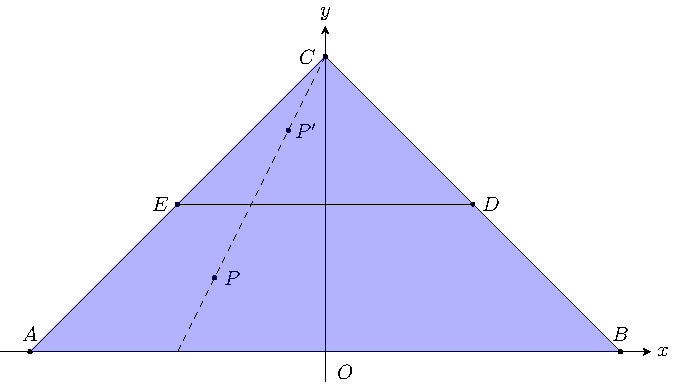
\includegraphics[scale=1]{images/fig_5.pdf}
                \end{center}
                \caption{Trapezoide $ABDE$.}
            \end{figure}
            y tomaremos a $E_2$ como el triángulo $ABC$. Definiremos una función $\cf{f}{E_1}{E_2}$ tal que el segmento $DE$ de la frontera de $E_1$ sea mapeada al vértice $C$ de $E_2$, pero en todos sus demás puntos sea una función biyectiva.

            Completaremos entonces la prueba diciendo que la topología cociente determinada por $f$ es la misma que la topología de $E_2$, esto para verificar que el espacio cociente de $E_1$ con su segmento es isomorfo a $E_2$, obteniendo así el resultado deseado.
            \item Definimos $f$ con la condición de que para todo $P=(x,y)\in E_1$, el punto $f(x,y)=P'=(x',y')\in E_2$ sea tal que esté en la recta que une a $P$ con $C=(0,1)$, dada de la siguiente manera:
            \begin{equation*}
                f(x,y)=\left(x\cdot\left(\frac{2y-1}{y-1}\right),2y \right)=(x',y'),\quad\forall (x,y)\in E_1
            \end{equation*}
            se verifica rápidamente que $g$ tiene como inversa en el conjunto $E_1$ menos el segmento $DE$ a la función $\cf{g}{E_2\setminus\left\{(0,1)\right\} }{E_1\setminus DE}$ dada por:
            \begin{equation*}
                g(x',y')=\left(x'\cdot\left(\frac{y'-2}{2y'-2} \right), \frac{1}{2}y'\right)=(x,y),\quad\forall (x',y')\in E_2\setminus\left\{(0,1) \right\} 
            \end{equation*}
            Es claro que $f$ es continua y que $g$ es la \textit{inversa} de $f$. Como $E_1$ es compacto y $E_2$ es Hausdorff, entonces $f$ es cerrada. Luego $E_2$ tiene la topología cociente inducida por $f$.
        \end{itemize}
    \end{proof}

    Estamos ahora listos para probar un lema fundamental. Sea $\cf{g}{I}{\mathbb{S}^1}$ (donde $\mathbb{S}^1$ denota la frontera de $\mathbb{D}^2$) la funcioń continua que da exactamente una vuelta alrededor del círculo, esto es
    \begin{equation*}
        g(0)=g(1)=d_0\in\mathbb{S}^1
    \end{equation*}
    esto es, que $g$ mapea el intervalo $(0,1)$ de forma homeomorfa en $B\setminus\left\{d_0 \right\}$.

    \begin{lema}
        Sea $X$ un espacio topológico. Una funcioń continua $\cf{f}{\mathbb{S}^1}{X}$ puede ser extendida a una función $\cf{F}{\mathbb{D}^2}{X}$ si y sólo si el bucle cerrado $\cf{f\circ g}{I}{X}$ es equivalente al bucle constante con punto base $f(d_0)$.
    \end{lema}

    \begin{proof}
        $\Rightarrow):$ Suponga que $\cf{f}{\mathbb{S}^1}{X}$ puede ser extendida a una función $\cf{F}{\mathbb{D}^2}{X}$. Considere el cuadrado unitario:
        \begin{equation*}
            S=\left\{ (x,y)\in\mathbb{R}^2\Big|0\leq x\leq 1\textup{ y }0\leq y\leq 1 \right\}
        \end{equation*}
        Definimos una función continua $\cf{h}{S}{\mathbb{S}^1}$ dada como sigue:
        \begin{equation*}
            \begin{split}
                h(x,0) &= g(x) \textup{ si } 0\leq x\leq 1\\
                h(x,1) &= h(0,y)=h(1,y)=d_0,\textup{ si }x\in I\textup{ o }y\in I \\
            \end{split}
        \end{equation*}
        Es claro que $h$ es continua. Por la proposición \ref{propB}, como $S\cong\mathbb{S}^1$, podemos extender $h$ a una función continua $\cf{H}{S}{\mathbb{S}^1}$. La función continua $\cf{F\circ H}{I\times I}{X}$ satisface que:
        \begin{equation*}
            \begin{split}
                F\circ H(x,0) &= F(h(x,0))\\
                &= F(g(x))\\
                &= f\circ g(x)\\
            \end{split}
        \end{equation*}
        y,
        \begin{equation*}
            \begin{split}
                F\circ H(x,1) &= F(h(x,1))\\
                &= F(d_0)\\
                &= f(d_0)\\
            \end{split}
        \end{equation*}
        para todo $x\in I$. Además,
        \begin{equation*}
            \begin{split}
                F\circ H(0,y) &= F(d_0) \\
                &= f(d_0)\\
            \end{split}
        \end{equation*}
        y,
        \begin{equation*}
            \begin{split}
                F\circ H(1,y) &= F(d_0) \\
                &= f(d_0)\\
            \end{split}
        \end{equation*}
        Por tanto, el bucle $f\circ g$ es equivalente al bucle constante con punto base $f(d_0)$.

        $\Leftarrow):$ Suponga que el bucle cerrado $f\circ g$ es equivalente al bucle constante con punto base $f(d_0)$. Entonces, existe una función continua $\cf{G}{I\times I}{X}$ tal que:
        \begin{equation*}
            \left\{
                \begin{split}
                    G(x,0) & = f\circ g(x)\\
                    G(x,1) & = G(0,y) = G(1,y) = f(d_0)\\
                \end{split}
            \right.,\quad\forall x\in I\textup{ y }\forall y\in I
        \end{equation*}
        notemos que de la segunda condición, $G$ mapea el borde superior y los dos bordes de $I\times I$ en un sólo punto, $f(d_0)$ en $X$, luego $G$ induce una función continua de este espacio cociente a $X$. Por la proposición anterior, este espacio cociente es un disco cerrado, digamos $\mathbb{D}^2$. Así que la función inducida $\cf{\widetilde{G}}{\mathbb{D}^2}{X}$ es tal que en un punto de de la frontera de $\mathbb{D}^2$, digamos $(x_0,y_0)\in\mathbb{D}^2$ se cumple que:
        \begin{equation*}
            \begin{split}
                \widetilde{G}(x_0,y_0)=f(d_0)
            \end{split}
        \end{equation*}
        y,
        \begin{equation*}
            \widetilde{G}(x,y)=f\circ g(x,y)
        \end{equation*}
        para todo $(x,y)\in\mathbb{S}^2\setminus\left\{(x_0,y_0)\right\}=I$. Por ende, $G$ es una extensión continua de $f$ a todo $\mathbb{D}^2$. 
    \end{proof}

    Aplicando el lema anterior, es conveniente usar el siguiente abuso de notación, diremos que la función $\cf{f}{\mathbb{S}^1}{X}$ \textit{representa} la clase de equivalencia del bucle $f\circ g$.

    \begin{theor}
        Sean $X$ y $Y$ espacios topológicos, $\cf{\varphi_0,\varphi_1}{X}{Y}$ funciones continuas homotópicas y sea $\cf{\varphi}{X\times I}{Y}$ la homotopía entre ambas funciones. Sea $x_0\in X$ y considere los homomorfismos inducidos por $\varphi_0$ y $\varphi_1$:
        \begin{equation*}
            \left\{
            \begin{split}
                &\cf{{\varphi_0}_*}{\pi(X,x_0)}{\pi(Y,\varphi_0(x_0))}\\
                &\cf{{\varphi_1}_* }{\pi(X,x_0)}{\pi(Y,\varphi_1(x_0))}\\
            \end{split}
            \right.
        \end{equation*}
        Sea $[\gamma]$ la clase de equivalencia del camino $\cf{\gamma}{I}{Y}$, dado por $t\mapsto\varphi_0(x_0,t)$. Considere el isomorfismo inducido $\cf{u}{\pi(Y,\varphi_0(x_0))}{\pi(Y,\varphi_1(x_0))}$ dado por:
        \begin{equation*}
            u([f])=[\gamma]^{-1}\cdot[f]\cdot[\gamma],\quad\forall [f]\in\pi(Y,\varphi_0(x_0))
        \end{equation*}
        Entonces, el diagrama

        \begin{minipage}{\textwidth}
            \begin{center}
                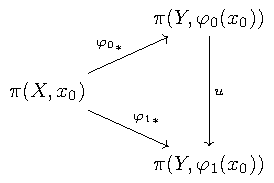
\includegraphics[scale=1.5]{images/fig_4.pdf}\\
                Figura 2: Conmutatividad de $\pi(X,x_0)$, $\pi(Y,\varphi_0(x_0))$ y $\pi(Y,\varphi_1(x_0))$.
            \end{center}
        \end{minipage}
        \stepcounter{figure}

        es conmutativo.
    \end{theor}

    \begin{proof}
        Tenemos que probar que
        \begin{equation*}
            {\varphi_1}_*\left([f]\right)=[\gamma]^{-1}\cdot{\varphi_0}_*\left([f]\right)\cdot[\gamma],\quad\forall [f]\in\pi(X,x_0)
        \end{equation*}
        En efecto, sea $[f]\in\pi(X,x_0)$. Considere la función $\cf{F}{I\times I}{Y}$ dada por:
        \begin{equation*}
            F(x,y)=\varphi(f(x),y),\quad\forall x,y\in I
        \end{equation*}
        esta función es continua por ser composición de funciones continuas. Observemos que:
        \begin{equation*}
            \left\{ 
                \begin{split}
                    F(x,0) & = \varphi(f(x),0)=\varphi_0(f(x)) \\
                    F(x,1) & = \varphi(f(x),1)=\varphi_1(f(x)) \\
                \end{split}
            \right.,\quad\forall x\in I
        \end{equation*}
        y,
        \begin{equation*}
            F(0,y)=F(1,y)=F(x_0,y)=\gamma(y),\quad\forall y\in I
        \end{equation*}
        Por ende, se tiene que el producto
        \begin{equation*}
            \left(\varphi_0\circ f \right)\cdot\gamma\cdot\left(\varphi_1\circ f \right)^{-1}\cdot\gamma^{-1}
        \end{equation*}
        es un bucle que va de la frontera de $I\times I$ (que se denotará por $\mathbb{S}^1$) a $Y$, esto es que es en algún sentido la función $\cf{F\big|_{\mathbb{S}^1}}{\mathbb{S}^1}{Y}$, la cual puede ser extendida de forma continua a $F$, así, por el lema anterior, se sigue que el camino $\left(\varphi_0\circ f \right)\cdot\gamma\cdot\left(\varphi_1\circ f \right)^{-1}\cdot\gamma^{-1}$ es equivalente al camino constante, es decir que:
        \begin{equation*}
            [\left(\varphi_0\circ f \right)\cdot\gamma\cdot\left(\varphi_1\circ f \right)^{-1}\cdot\gamma^{-1}]=e
        \end{equation*}
        esto es, que
        \begin{equation*}
            \begin{split}
                {\varphi_0}_*\left([f]\right)\cdot[\gamma]&=[\gamma]\cdot{\varphi_1}_*\left([f]\right)\\
                \Rightarrow {\varphi_1}_*\left([f]\right)&=[\gamma]^{-1}\cdot{\varphi_0}_*\left([f]\right)\cdot[\gamma]\\
            \end{split}
        \end{equation*}
        lo cual prueba el resultado.
    \end{proof}

    Note que este teorema es una generalización de un teorema anterior. 

    \begin{mydef}
        Dos espacios topológicos $X$ y $Y$ tienen el \textbf{mismo tipo de homotopía} si existen funciones continuas, llamadas \textbf{equivalencias de homotopía}, $\cf{f}{X}{Y}$ y $\cf{g}{Y}{X}$ tales que:
        \begin{equation*}
            g\circ f\simeq\bbm{1}_X\quad\textup{y}\quad f\circ g\simeq\bbm{1}_Y
        \end{equation*}
    \end{mydef}

    Se sigue de forma inmediata que dos espacios homeomorfos tienen el mismo tipo de homotopía, pero el converso no es cierto (en general).

    \begin{theor}
        Si $\cf{f}{X}{Y}$ es una equivalencia de homotopía, entonces $\cf{f_*}{\pi(X,x)}{\pi(Y,f(x))}$ es un isomorfismo para todo $x\in X$.
    \end{theor}

    \begin{proof}

        Como $f$ es equivalencia de homotopía, existe una función $\cf{g}{Y}{X}$ tal que
        \begin{equation*}
            f\circ g\simeq\bbm{1}_Y\quad\textup{y}\quad g\circ f\simeq\bbm{1}_X
        \end{equation*}
        Por el lema anterior y usando las propiedades de los homomorfismos inducidos, obtenemos los siguientes dos diagramas conmutativos.

        \begin{figure}
            \begin{center}
                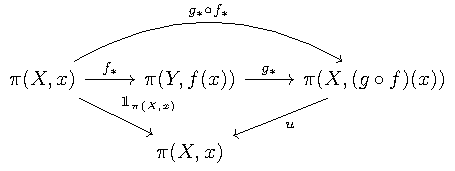
\includegraphics[scale=1.5]{images/fig_6.pdf}
            \end{center}
            \caption{Diagrama Conmutativo de $\bbm{1}_{\pi(X,x)}$, $g_*\circ f_*$ y $u$.}
        \end{figure}

        \begin{figure}
            \begin{center}
                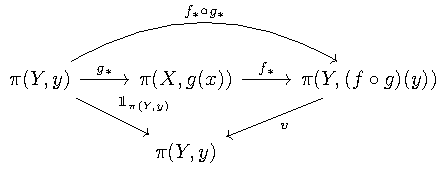
\includegraphics[scale=1.5]{images/fig_7.pdf}
            \end{center}
            \caption{Diagrama Conmutativo de $\bbm{1}_{\pi(Y,y)}$, $f_*\circ g_*$ y $v$.}
        \end{figure}

        Estos son válidos para todo $x\in X$ y para todo $y\in Y$, donde las funciones $u$ y $v$ son como las dadas en el Teorema anterior para algún caminos que las definan. En particular, obtenemos que:
        \begin{equation*}
            u\circ (g_*\circ f_*) =\bbm{1}_{\pi(X,x)}\quad\textup{y}\quad v\circ (f_*\circ g_*)=\bbm{1}_{\pi(Y,y)}
        \end{equation*}
        donde $u$ y $v$ son isomorfismos, luego de forma inmediata se sigue que $f_*$ y $g_*$ también deben de serlo (restringidos a los dominios adecuados).
    \end{proof}

    Este teorema será usado como mira para determinar los grupos fundamentales de ciertos espacios, y como un método de probar que ciertos espacios no tienen el mismo tipo de homotopía (y en consecuencia, no son homeomorfos).

\end{document}